\chapter{Clustering}

\section{Evaluation of a new instance}

At this point, with a model trained on the data, a generic $n$th new snapshot instance $\vect{\mathcal{S}}_n$ can be evaluated using the K-means algorithm.
From a geometric point of view, the snapshot $\vect{\mathcal{S}}_n$ is a point in the ${F}$-dimensional space, where ${F}$ is the number of features used to train the model.

For demonstration purposes, in this section, it is considered an example with ${F}=3$ features.

\begin{figure}[htbp]
  \centering
  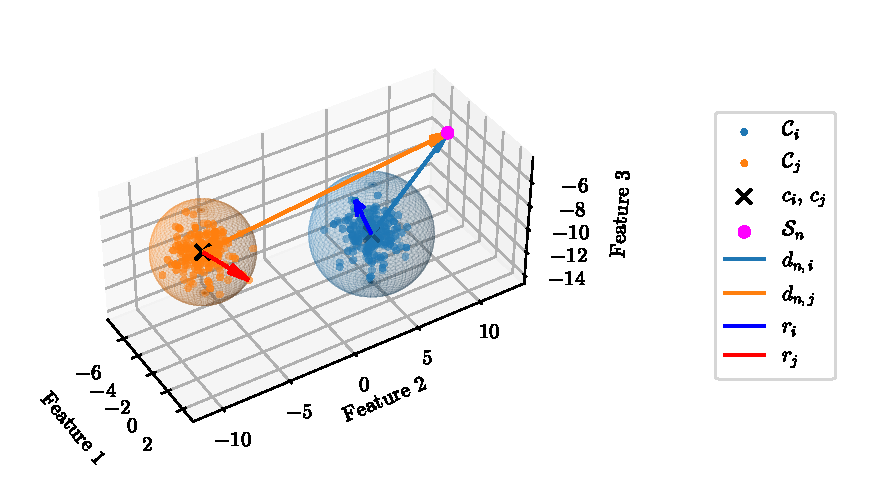
\includegraphics[width=\textwidth]{images/Spheres_2.pdf}
\caption{Cluster model in the $3$-dimensional space, with new snapshot $\vect{\mathcal{S}}_n$}
\label{fig:clust_spheres}
\end{figure}

In the \autoref{fig:clust_spheres}, the training data are represented in the $3$-dimensional space, where the axis are the features used to train the model. The K-means model has been ideally trained with an arbitrary number $k$ of clusters but, for display purposes, only two clusters  ($\vect{\mathcal{C}}_i$ and $\vect{\mathcal{C}}_j$) are plotted. 
\paragraph*{}
The entities shown in the \autoref{fig:clust_spheres} are:
\begin{itemize}
  \item $\vect{c}_{i(j)}$ is the centroid of the $i$th ($j$th) cluster;
  \item $\vect{r}_{i(j)}$ is the radius of the $i$th ($j$th) cluster, it is defined as the distance between the centroid $\vect{c}_{i(j)}$ and the farthest point belonging to the cluster itself;
  \item $\vect{\mathcal{C}}_{i(j)}$ is the set of training snapshots belonging to the $i$th ($j$th) cluster, it has a centroid $\vect{c}_{i(j)}$ and a radius $\vect{r}_{i(j)}$;
  \item $\vect{\mathcal{S}}_n$ is the new snapshot to be evaluated;
  \item $\vect{d}_{n,i}$ is the distance between $\vect{\mathcal{S}}_n$ and $\vect{c}_i$;
  \item $\vect{d}_{n,j}$ is the distance between $\vect{\mathcal{S}}_n$ and $\vect{c}_j$;
\end{itemize}

\subsection{Assignation of the new instance to a cluster} 
The procedure for assigning the new snapshot $\vect{\mathcal{S}}_n$ to a cluster is quite simple, it is sufficient to compute the distance between $\vect{\mathcal{S}}_n$ and the centroids $\vect{c}_m$, $\forall m \in  [1, \dots , k]$. The distance is defined as the $l^2$-norm in the feature space, and can be computed using the \autoref{eq:clust_dist}, and assign $\vect{\mathcal{S}}_n$ to the cluster with the minimum distance.

\begin{equation}
  \label{eq:clust_dist}
  \vect{d}_{n,m} = ||\vect{\mathcal{S}}_{n,f} - \vect{c}_{m,f}||_2 = \sqrt{\sum_{f=1}^{F} (\vect{\mathcal{S}}_{n,f} - \vect{c}_{m,f})^2}
\end{equation}

\subsection{Evaluation of the new instance}
Once the new snapshot $\vect{\mathcal{S}}_n$ has been assigned to the right cluster $\vect{\mathcal{C}}_i$, some kind of measure linked to how novel this snapshot is need to be computed. In this document, this measure, referred to the $n$-th cluster, will be called $e_n$, in order to remind some sort of error, even if it is not an error in the strict sense. One simple approach could be to compute the disfference between the distance of $\vect{\mathcal{S}}_n$ from the centroid $\vect{c}_i$ and the radius $\vect{r}_i$ of the cluster itself. With this approach, the measure defined in the \autoref{eq:clust_eval} is relative to the current snapshot, so it is possible to use that as a novelty measure.

Few consideration about the resoult of the \autoref{eq:clust_eval}:
\begin{itemize}
  \item if $\vect{e}_{n} > 0$, the new snapshot $\vect{\mathcal{S}}_n$ is outside the sphere of radius $\vect{r}_i$ centered in $\vect{c}_i$, so it is probably a novel snapshot;
  \item if $\vect{e}_{n} < 0$, the new snapshot $\vect{\mathcal{S}}_n$ is inside the sphere of radius $\vect{r}_i$, so it is probably a normal snapshot. In this case it is worth noticing that this assumption is reasonable only if the shape of the point cloud resambles a sphere, otherwise the radius $\vect{r}_i$ is not a good measure of the cluster size, and use it for novelty detection would not be reasonable. \emph{This enpasises the importance of the standardization procedure applied to the features before the training phase};
\end{itemize}

\begin{equation}
  \label{eq:clust_eval}
  \vect{e}_{n} = ||\vect{d}_{n,i}||_2 - ||\vect{r}_{i}||_2, \text{ where $i$ is the of the assigned cluster}
\end{equation}


